\subsection{Aire Guru}

Aire Guru utiliza los datos de calidad del aire proporcionados por el ayuntamiento de Malaga en su portal de datos abiertos.\footnote{\url{https://datosabiertos.malaga.eu/}}
\begin{figure}[h]
    \centering
   \subfigure[Pagina principal]
    {\includegraphics[width=5.5cm  ]{OpenDataPortal}}
    \hfill
    \subfigure [Categoria medio ambiente]
       { 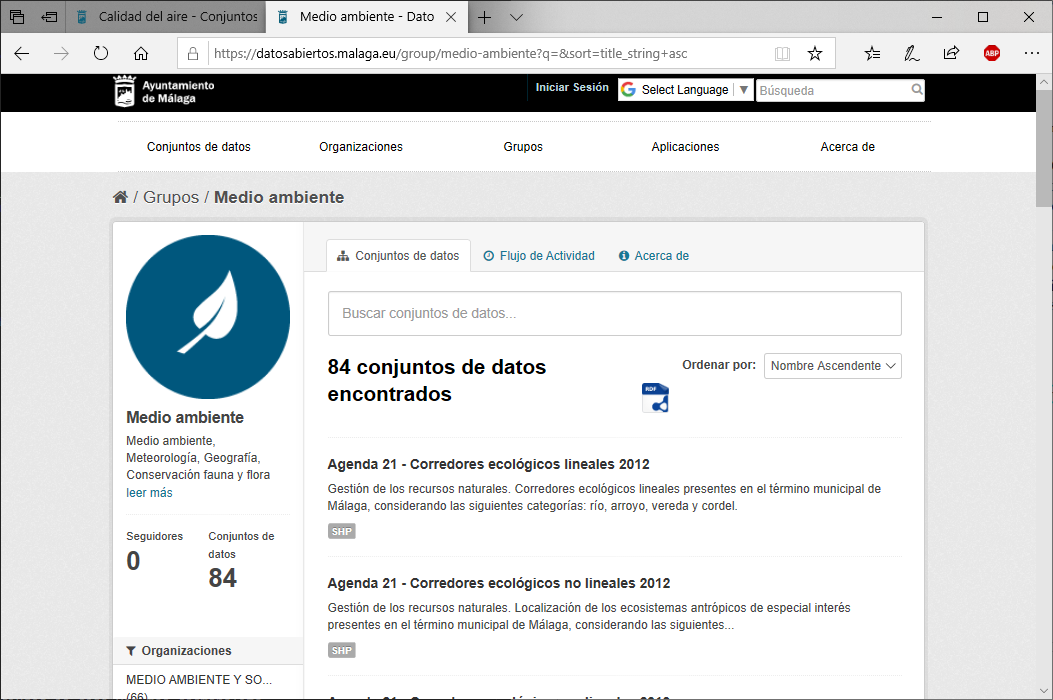
\includegraphics[width=5.5cm]{openDataPortalEnviromentCategory}}
  
  \caption{Open Data Portal Malaga}
    \end{figure}
Este portal de datos ofrece una oferta de categorias representados por iconos, por lo que es necesario saber en que categoria se clasifica el conjunto
de datos, una vez que se accede a la categoria, tenemos una barra buscadora que nos permite insertar las palabras claves para buscar el conjunto de datos
deseado.\\

Los datos extraidos estan en formato GeoJSON, este formato proporciona un objeto JSON con subdocumentos anidados, cada uno de estos
subdocumentos contiene un conjunto de datos en forma clave valor. 
En la siguiente figura podemos ver el principio del documento descargado el 09 de Junio del 2019 
\footnote{\url{https://datosabiertos.malaga.eu/recursos/ambiente/calidadaire/calidadaire.json}}\\
\newpage
\begin{figure}[h]
    \centering
   \subfigure[Primer subdocumento]{ \centering 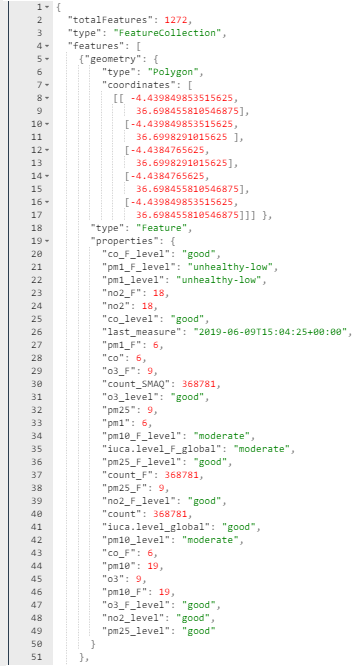
\includegraphics[width=4.75cm]{geoJsonAirQualityData1}}
   \hfill
   \subfigure[Segundo subdocumento]{ \centering 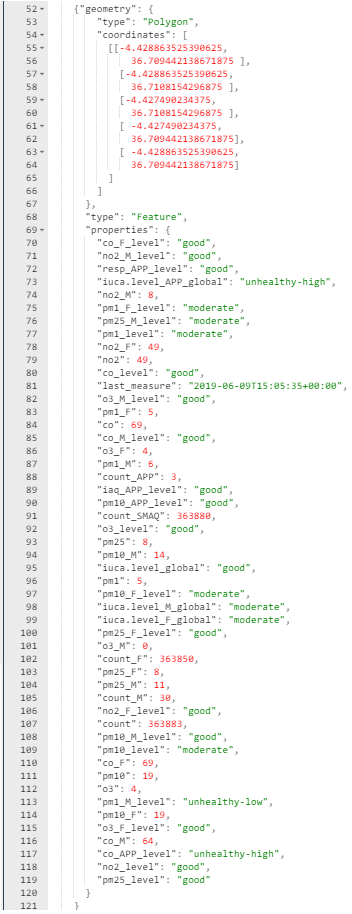
\includegraphics[width=4.75cm]{geoJsonAirQualityData2}}
    \caption{Air quality Document [09/06/2019].Open Data Portal Malaga}
    \end{figure}
    
En este extracto podemos ver los primeros dos subdocumentos. Cada subdocumento contiene las coordenadas de la estacion medidora de la calidad
del aire, la fecha y hora cuando se registro la medida y a continuacion los valores de las mediciones. 
En la figura siguiente podemos encontrar la descripcion proporcionada por el portal de datos abiertos.
\begin{figure}[ht]
    \centering
    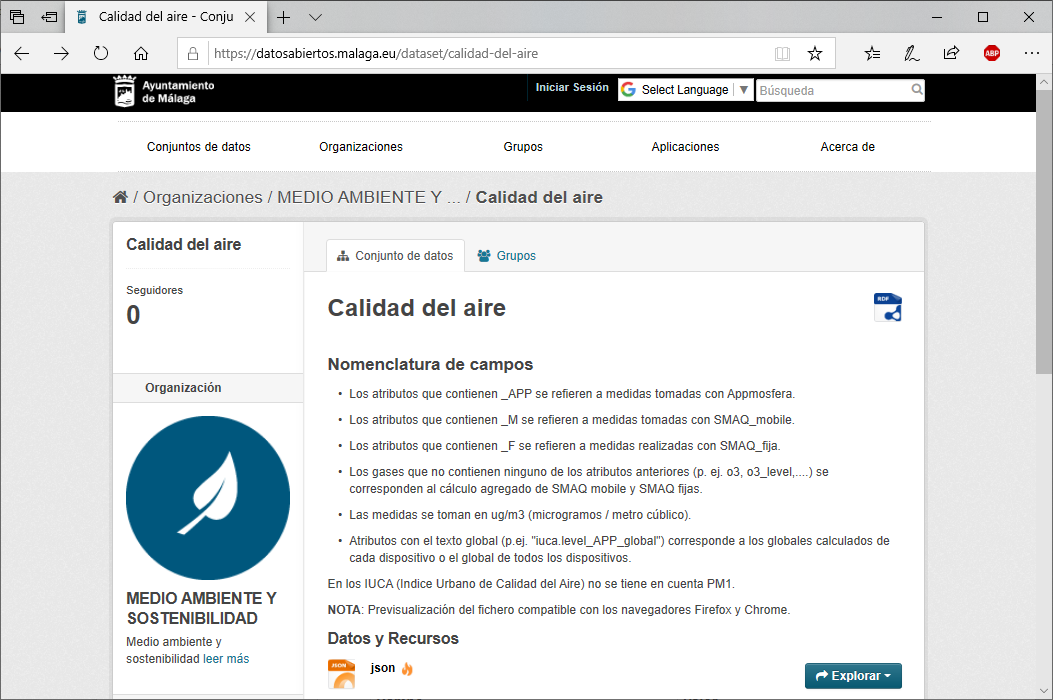
\includegraphics[width=8cm]{geoJsonAirQualityDataDescription}
    \caption{Air quality data description [09/06/2019].Open Data Portal Malaga}
\end{figure}

Para una descripcion mas en detalle de las medidas, tenemos que recurrir a un recurso externo, en este caso nos pusimos en contacto directamente con
la empresa que instala las estaciones de medida UrbanClouds \footnote{\url{https://urbanclouds.city/es/}} y proporciona los datos al ayuntamiento de Malaga.

La herramienta Aire guru presenta la informacion en el idioma nativo de la ciudad y actualmente se esta trabajando en su traduccion 
al ingles, para cubrir un rango mas amplio de su poblacion, ya que esta ciudad es cada vez mas cosmopolita.
Se utiliza un lenguaje sencillo y directo y se acompana de pictogramas, facil de identificar, para una
lectura mas rapida de la situacion.



--acceso a los datos
Aire Guru esta disponible al usuario mediante la url segura https://www.aire.guru y https://www.airquality.guru.
El uso de SSL proporciona ademas de 
--navegadores
una opcion segura para los usuarias, ya que asegura en envio de informacion a traves de la red de forma
cifrada.
Para acceder a la informacion general
--lectura familiar de los datos
iconografia
colores oficiales
